\label{sec-results}

A execução completa gerou a representação final de 18 features para 100.694
batimentos válidos. A SVM supervisionada foi treinada com os 51.002 batimentos
de DS1, enquanto a One-Class SVM recebeu apenas os 38.088 batimentos normais
desse mesmo conjunto. O teste em DS2 manteve 49.692 batimentos, com
36.428 normais e 13.264 anômalos. A
Tabela~\ref{tab-final-metrics} resume a comparação principal.

\begin{table*}[!htbp]
  \centering
  \caption{Resultados da comparação inter-paciente para a representação final.}
  \label{tab-final-metrics}
  \small
  \renewcommand{\arraystretch}{1.10}
  \begin{tabular}{lp{3.8cm}rrrrrr}
    \toprule
    Modelo & Treino & Features & PR-AUC & ROC-AUC & Precision & Recall & F1 \\
    \midrule
    SVM supervisionada & normais + anômalos de DS1 & 18 & 0.528 & 0.748 & 0.485 & 0.358 & 0.412 \\
    One-Class SVM & apenas normais de DS1 & 18 & 0.448 & 0.537 & 0.354 & 0.388 & 0.370 \\
    \bottomrule
  \end{tabular}
  \renewcommand{\arraystretch}{1.0}
\end{table*}

A SVM supervisionada superou a One-Class SVM em PR-AUC, ROC-AUC, precision e
F1 na mesma representação final. A diferença de 0,080 ponto de PR-AUC mostra
vantagem consistente do regime supervisionado quando há rótulos anômalos
disponíveis no treino. A Figura~\ref{fig-pr-curves} mostra que essa vantagem
não depende apenas de um limiar específico, pois a SVM mantém precision mais
alta ao longo da maior parte da faixa de recall observada.

\begin{figure}[H]
  \centering
  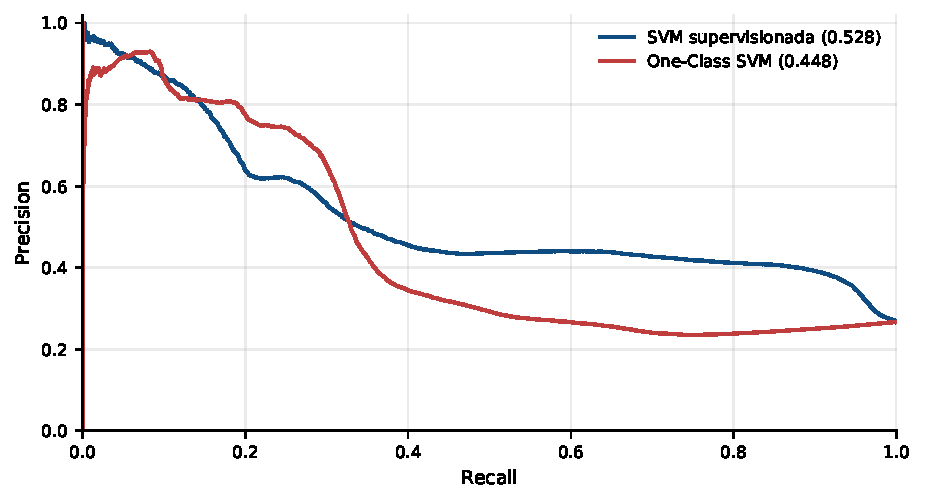
\includegraphics[width=0.72\linewidth]{figures/fig_model_precision_recall.pdf}
  \caption{Curvas precision-recall da SVM supervisionada e da One-Class SVM no teste inter-paciente.}
  \label{fig-pr-curves}
\end{figure}

O limiar operacional destaca um trade-off diferente entre os modelos. A
One-Class SVM recuperou 5153 anomalias no teste, enquanto a SVM supervisionada
recuperou 4753. Esse ganho de 400 verdadeiros positivos veio acompanhado de
4379 falsos positivos adicionais. A queda de precision para 0,354, frente a
0,485 na SVM supervisionada, confirma que a fronteira one-class operou de forma
mais permissiva no conjunto inter-paciente.

\begin{table}[H]
  \centering
  \caption{Matrizes de confusão no teste inter-paciente.}
  \label{tab-confusion-matrices}
  \small
  \renewcommand{\arraystretch}{1.10}
  \begin{tabular}{lrrrr}
    \toprule
    Modelo & TN & FP & FN & TP \\
    \midrule
    SVM supervisionada & 31385 & 5043 & 8511 & 4753 \\
    One-Class SVM & 27006 & 9422 & 8111 & 5153 \\
    \bottomrule
  \end{tabular}
  \renewcommand{\arraystretch}{1.0}
\end{table}

\begin{figure}[H]
  \centering
  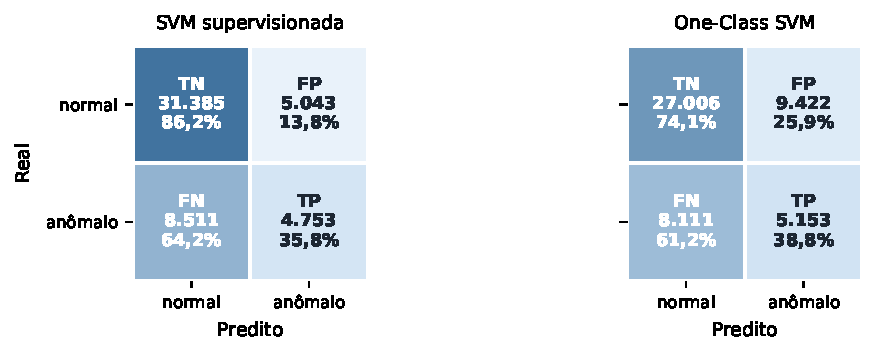
\includegraphics[width=0.84\linewidth]{figures/fig_confusion_matrices.pdf}
  \caption{Matrizes de confusão visualizadas por proporção em cada classe real. Cada célula mostra o tipo de acerto ou erro, a contagem e o percentual da linha correspondente.}
  \label{fig-confusion-heatmaps}
\end{figure}

As matrizes de confusão da Tabela~\ref{tab-confusion-matrices} e da
Figura~\ref{fig-confusion-heatmaps} tornam esse contraste mais direto. Entre os
batimentos normais, a SVM supervisionada manteve 86,2\% classificados como
normais, contra 74,1\% na One-Class SVM. Entre os batimentos anômalos, a
One-Class SVM reconheceu 38,8\%, contra 35,8\% na SVM supervisionada. A pequena
vantagem de recall da formulação one-class veio acompanhada de perda expressiva
de especificidade.
\FloatBarrier
